\documentclass[12pt,a4paper]{article}

\usepackage{amsfonts}
\usepackage{amsmath}
%\usepackage[centertags]{amsmath}
%\usepackage{german}
\usepackage{amsthm}
\usepackage{amsmath}
\usepackage{mathtools}
\usepackage{amssymb}
\usepackage{tikz}
\usepackage{tikz-cd}
\usetikzlibrary{matrix,arrows}
\usepackage[english, ngerman]{babel}
\usepackage[utf8]{inputenc}
\usepackage[T1]{fontenc}
\usepackage{hyperref}
\usepackage{cite}
\usepackage[nottoc,numbib]{tocbibind}


\leftmargin=0pt \topmargin=0pt \headheight=0in \headsep=0in \oddsidemargin=0pt \textwidth=6.5in
\textheight=8.5in


\newcommand{\eps}{\varepsilon}
\renewcommand{\phi}{\varphi}
\newcommand{\Sl}{\ell}    % schönes l
\newcommand{\ve}{\varepsilon}  %Epsilon

% Theorem Stil

\theoremstyle{plain}
\newtheorem{lem}{Lemma}[section]
\newtheorem{lem*}{Lemma}
\newtheorem{prop}[lem]{Proposition}
\newtheorem{thm}[lem]{Theorem}
\newtheorem{cor}[lem]{Corollary}

\theoremstyle{definition}
\newtheorem{defn}[lem]{Definition}
\newtheorem*{ex}{Example}

\theoremstyle{remark}
\newtheorem{rem}{Bemerkung}    %[section]

\newcommand{\card}{\mathop{\rm card}\nolimits}
\newcommand{\Sets}{((Sets))}
\newcommand{\id}{{\rm id}}
\newcommand{\supp}{\mathop{\rm Supp}\nolimits}

\newcommand{\nin}{\notin}
\newcommand{\ord}{\mathop{\rm ord}\nolimits}
\renewcommand{\mod}{\mathop{\rm mod}\nolimits}
\newcommand{\sign}{\mathop{\rm sign}\nolimits}
\newcommand{\height}{\mathop{\rm height}\nolimits}
\newcommand{\ggT}{\mathop{\rm ggT}\nolimits}
\newcommand{\kgV}{\mathop{\rm kgV}\nolimits}
\renewcommand{\div}{\, | \,}
\newcommand{\nequiv}{\not \equiv}
\newcommand{\notdiv}{\mathopen{\mathchoice
             {\not{|}\,}
             {\not{|}\,}
             {\!\not{\:|}}
             {\not{|}}
             }}


\newcommand{\quotient}[2]{
        \mathchoice
            {% \displaystyle
                \text{\raise1ex\hbox{$#1$}\Big/\lower1ex\hbox{$#2$}}%
            }
            {% \textstyle
                #1\,/\,#2
            }
            {% \scriptstyle
                #1\,/\,#2
            }
            {% \scriptscriptstyle  
                #1\,/\,#2
            }
    }
		
\newcommand{\doublequotient}[4]{\quotient{\textstyle \left( \quotient{$#1$}{$#2$} \right)}{\textstyle \left( \quotient{$#3$}{$#4$} \right)}}


\renewcommand{\binom}[2]{\left({#1}\atop{#2}\right)}
\newcommand{\eck}[1]{\langle #1 \rangle}
\newcommand{\gaussk}[1]{\lfloor #1 \rfloor}
\newcommand{\frack}[1]{\{ #1 \}}
\newcommand{\wi}{\hspace{1pt} < \hspace{-6pt} ) \hspace{2pt}}
\newcommand{\dreieck}{\bigtriangleup}
\newcommand{\R}{\mathbb{R}}

\parindent0mm


\begin{document}

\pagestyle{empty}

\begin{center}
{\huge Lösungen zur IMO-Selektionsprüfung 2014} \\
\end{center}
\vspace{8mm}

\begin{enumerate}
     \item[\textbf{1.}]Trouver toutes les fonctions $f: \mathbb{N}\to \mathbb{N}$ telles que pour tous $m,n\in \mathbb{N}$, on ait
\[
m^2+f(n)|mf(m)+n
\]

\textit{$1^{ere}$solution:}\\
Avec $m=n$, on obtient $m^2+f(m)|mf(m)+m$.
\[\Rightarrow m^2+f(m)|mf(m)+m -m(m^2+f(m)) \Rightarrow m^2+f(m)|m^3-m\]
Donc, avec $m=2$, on a $4+f(2)|6$ et comme $f(2)>0$, on a $f(2)=2$.\\
Substituons $m=2$ au départ, on a $4+f(n)|4+n$ et donc $n \geq f(n)$, $\forall n \in \mathbb{N}$. 
En particulier, $0<f(1)\leq 1$ et donc $f(1)=1.$\\
De plus, on a $m^2+f(m)|mf(m)+m$, et donc $f(m) \geq m$, $\forall m \in \mathbb{N}-\{1\}$.\\
On en conclut que $f(n)=n$, $\forall n \in \mathbb{N}$, qui est bien une solution.

\textit{$2^{eme}$solution:}\\
Posons $m=f(n)$, on obtient $f(n)^2 +f(n) | f(n)f(f(n)) + n$ et donc $f(n)|n$. 
En particulier, $f(n)\leq n$ $\forall n \in \mathbb{N}$ et $f(1)=1$.\\
En posant $n=1$, on obtient $m \leq f(m)$,  $\forall m \in \mathbb{N}$.
On conlcut de la męme maničre.

	
\item[\textbf{2.}] Gegeben sind $2n$ Chips, die in einer Reihe liegen. In einem Zug kann man zwei benachbarte Chips vertauschen. Wieviele Züge muss man machen, damit jeder Chip einmal am Anfang und einmal am Ende der Reihe war?\\
	
\textit{Lösung:}\\
Man muss insgesamt $3n^2-2n$ Züge machen.\\
Untere Schranke:\\
Wir zählen, wie oft alle Chips zusammen um eins verschoben werden müssen.\\
Jeder Chip wird sicher von seiner Anfangsposition bis zum näheren Rand, vom einen Rand zum anderen Rand und vom anderen Rand zu seiner Endposition verschoben. Ein Chip an der Position $i$ muss bis zum näheren Rand $i-1$ respektive $2n-i$ verschoben werden. Da am Anfang alle Positionen besetzt sind, müssen alle Chips zusammen von ihren Anfangspositionen zum je näheren Rand mindestens $\sum_{i=1}^n (i-1)+\sum_{i=n+1}^{2n} (2n-i)=2 \sum_{i=1}^n (i-1)$ verschoben werden. Da am Ende ebenfalls alle Positionen besetzt sind, müssen alle Chips zusammen vom anderen Rand zur jeweiligen Endposition mindestens $2 \sum_{i=1}^n (i-1)$ verschoben werden. Dann muss jeder Chip noch vom einen Rand zum anderen Rand verschoben werden, pro Chip sind das $2n-1$ Verschiebungen, also insgesamt $2n(2n-1)$. Zusammengezählt gibt das auf $4 \sum_{i=1}^n (i-1)+2n(2n-1)=6n^2-4n$. Da ein Zug zwei Chips verschiebt, folgt daraus die gewünschte untere Schranke.\\
Konstruktion:\\
Idee: Wir schieben alle Chips auf der linken Hälfte zuerst zum linken Rand und alle Chips auf der rechten Hälfte zuerst zum rechten Rand. Dann vertauschen wir die beiden Hälften der Chips. Danach schicken wir jeden Chip noch zum jeweils anderen Rand.\\
Nun geben wir eine Konstruktion an, die dies macht, und zählen, wie viele Schritte wir dazu brauchen.\\
Der erste Chip ist schon am linken Rand. Den zweiten schicken wir mit einem Zug an den linken Rand, dann den dritten mit zwei Zügen, ... , und zuletzt noch den $n-1$ten mit $n-1$ Zügen. Dies gibt insgesamt $\sum_{i=1}^n (i-1)$. Wegen Symmetrie der Situation brauchen wir gleich viele Züge, um alle Chips auf der rechten Seite zum rechten Rand zu schieben.\\
Nun vertauschen wir die beiden Hälften der Chips. Dazu benennen wir die linke Hälfte der Chips mit $L_1, \dots, L_n$ und die rechte Hälfte mit $R_1, \dots R_n$ und wenden folgende Verschiebungen an:
\[
\begin{tabular}{|c|c|c|c|c|c|c|c|}\hline
$L_1 $&$ ...$&$ L_{n-2}$&$L_{n-1}$&$L_n $&$R_1$&$...$&$R_n$ \\ \hline
$L_1$&$...$&$L_{n-2}$&$L_{n-1}$&$R_1$&$...$&$R_n$&$L_n $\\ \hline
$L_1$&$...$&$L_{n-2}$&$R_1$&$...$&$R_n$&$L_{n-1}$&$L_{n}$ \\ \hline
...&...&...&...&...&...&...&... \\ \hline
$R_1$&$...$&$R_n$&$L_1 $&$ ...$&$ L_{n-2}$&$L_{n-1}$&$L_n$ \\ \hline
\end{tabular}
\]
Dies braucht insgesamt $n^2$ Züge, da jeder der $L_i$-Chips um $n$ nach rechts verschoben wird.\\
Nun müssen noch alle $L_i$-Chips den rechten Rand und alle $R_i$-Chips den linken Rand besuchen. Dies ist analog zur der Situation, als wir alle linken Chips zum linken und alle rechten Chips zum rechten Rand geschoben haben, braucht also insgesamt $2\sum_{i=1}^n (i-1)$ Züge.
Wir rechnen alle gebrauchten Züge zusammen und kommen wie beabsichtigt auf $3n^2-2n$.

\item[\textbf{3.}] Gegeben sind $4$ Punkte in der Ebene, sodass die $4$ Dreiecke, die sie aufspannen, alle denselben Inkreisradius haben. Zeige, dass die $4$ Dreiecke kongruent sind.\\
	
\textit{1. Lösung:}\\
Seien $A,B,C$ und $D$ die vier Punkte. Zuerst bemerken wir, dass $D$ ausserhalb des Dreiecks $ABC$ liegen muss, da sonst die Inkreise der anderen drei Dreiecke strikt kleinere Radius hätten als $ABC$. Wir können also o.B.d.A annehmen, dass $ABCD$ ein konvexes Viereck bilden. \\
Seien nun $I_1,I_2,I_3$ und $I_4$ die Inkreismittelpunkte der Dreiecke $DAB,ABC,BCD$ resp. $CDA$. Nach Voraussetzung ist jede Seite von $I_1I_2I_3I_4$ parallel zu einer von $ABCD$. Weiter definieren wir $X$ und $Y$ als die Lote von $I_1$ und $I_2$ auf die Strecke $AB$. Wiederum nach Voraussetzung gilt $I_1I_2 = XY$. Zudem haben wir
\[
AX = \frac{AB+AD-BD}{2} \text{ und } YB=\frac{BC+BA-AC}{2},
\]
also
\[
I_1I_2=XY = AB-AX-BY= \frac{BD+AC}{2} - \frac{AD+BC}{2}.
\]
Für $I_3I_4$ erhält man das selbe Resultat, wobei man in obigem Ausdruck $A$ mit $C$ und $B$ mit $D$ vertauschen muss, aber das ändert den Ausdruck offensichtlich nicht. Folglich gilt $I_1I_2=I_3I_4$ und analog auch $I_2I_3 = I_4I_1$, also ist $I_1I_2I_3I_4$ ein Parallelogramm, womit auch $ABCD$ eins sein muss.\\
Nun gilt für ein beliebiges Dreieck mit Fläche $F$, Umfang $U$ und Inkreisradius $r$ die Formel $F=\frac{Ur}{2}$. Da $ABCD$ ein Parallelogramm ist, haben $ABC$ und $ABD$ dieselbe Fläche und somit auch den selben Umfang. Wegen $BC=AD$ folgt also $AC=BD$. Folglich ist $ABCD$ ein Parallelogramm, in welchem beide Diagonalen gleich lang sind, also ein Rechteck. Die Aussage ist nun offensichtlich.\\

\textit{2. Lösung:}\\
Wir beweisen zunächst das folgende Lemma:

\begin{lem*}
Sind $ABC$ und $DEF$ zwei Dreiecke mit $AB=DE$, $\angle BAC>\angle EDF$ und $\angle CBA>\angle FED$, dann hat das Dreieck $ABC$ einen grösseren Inkreisradius.
\end{lem*}

\begin{proof}
Wir versetzen das Dreieck $DEF$ auf das Dreieck $ABC$, sodass $D$ auf $A$, $E$ auf $B$ und $F$ auf derselben Seite der Geraden $AB$ wie $C$ zu liegen kommt. Seien $I$ und $J$ die Inkreismittelpunkte der Dreiecke $ABC$ und $DEF$. Wegen $\angle BAI=\frac{1}{2}\angle BAC>\frac{1}{2}\angle EDF=\angle EDJ$ und $\angle IBA=\frac{1}{2}\angle CBA>\frac{1}{2}\angle FED=\angle JED$ liegt $J$ im Innern des Dreiecks $ABI$. Somit hat $I$ einen grösseren Abstand zur Seite $AB$ als $J$. Da diese Abstände aber gerade die Inkreisradien der Dreiecke $ABC$ und $DEF$ sind, folgt hieraus, dass das Dreieck $ABC$ einen grösseren Inkreisradius hat.
\end{proof}

\begin{rem}Wie man sich leicht überlegt, gilt das Lemma auch noch, wenn man bei einer der beiden Winkelungleichungen das Ungleichheitszeichen durch ein Gleichheitszeichen ersetzt.
\end{rem}

Wir nennen die 4 gegebenen Punkte $A,B,C$ und $D$. Aus dem Lemma folgt sofort, dass das Viereck $ABCD$ konvex sein muss.\\
Sei $r$ der Inkreisradius der 4 Dreiecke. In den folgenden Umformungen benutzen wir, dass die Fläche eines Dreiecks gleich gross ist wie die Hälfte des Produkts aus Inkreisradius und Umfang:
\begin{align*}
2[ABCD]&=2[ABCD]\\
2[ABC]+2[ACD]&=2[ABD]+2[DBC]\\
r\cdot(AB+BC+CA)+r\cdot(AC+CD+DA)&=r\cdot(AB+BD+DA)+r\cdot(DB+BC+CD)\\
AB+BC+CA+AC+CD+DA&=AB+BD+DA+DB+BC+CD\\
2AC&=2BD\\
AC&=BD
\end{align*}

\begin{figure}[htbp]
\centering 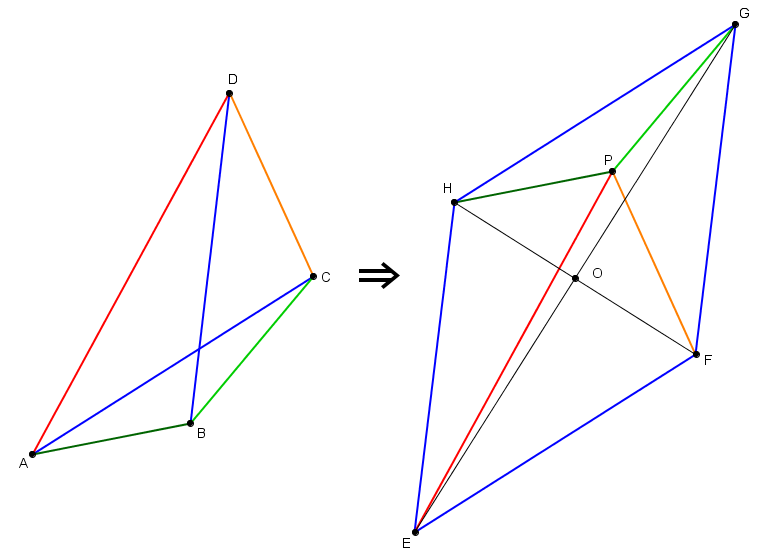
\includegraphics[width=0.60\textwidth]{Inkreis} \label{fig:Aufgabe3}
\end{figure}

Die Diagonalen des Vierecks $ABCD$ sind somit gleich lang. Wir setzen nun die 4 Dreiecke zu einer Raute $EFGH$ zusammen (siehe Abbildung). Nach Konstruktion der Raute gibt es im Innern einen Punkt $P$, sodass die Dreiecke $EFP$, $FGP$, $GHP$ und $HEP$ gerade Kopien der ursprünglichen Dreiecke sind. Wir wissen also, dass auch diese neuen Dreiecke denselben Inkreisradius besitzen.\\
Sei $O$ der Diagonalenschnittpunkt der Raute. Wenn wir zeigen können, dass $O=P$ gilt, sind wir fertig, denn jede Raute wird durch die Diagonalen in 4 kongruente Dreiecke unterteilt.\\
Angenommen, der Punkt $P$ liege im Innern des Dreiecks $OGH$. Dann gilt:
\[
\angle HGP<\angle HGO=\angle FEO<\angle FEP
\]
\[
\angle PHG<\angle OHG=\angle OFE<\angle PFE
\]
Wir können also das Lemma auf die Dreiecke $GHP$ und $EFP$ anwenden und erhalten, dass das Dreieck $EFP$ einen grösseren Inkreisradius besitzt, Widerspruch.\\
Analog kann gezeigt werden, dass $P$ auch nicht im Innern der anderen Dreiecke oder im Innern der Strecken $EO$, $FO$, $GO$ und $HO$ liegen kann. Somit folgt $P=O$ und wir sind fertig.
	
	
	\item[\textbf{4.}] Bestimme alle Polynome $P$ mit reellen Koeffizienten, sodass für alle $x \in\mathbb{R}$ gilt:
\[(x+2014)P(x)=xP(x+1)\]

\textit{Lösung:}\\
Setzt man $x=0$ sieht man, dass $P(0)=0$ gelten muss. Setzt man nun $x=-1$ folgt $P(-1)=0$ usw. Somit sehen wir, dass $0,-1,-2,\dots,-2013$ alles Nullstellen von $P$ sind. Wir zeigen nun, dass der Grad $n$ von $P$ genau $2014$ sein muss. Dazu schreiben wir $P(X) = a_nX^{n}+a_{n-1}X^{n-1}+\dots+a_1X+a_0$ mit $a_n \neq 0.$ Da beide Seiten der Gleichung Polynome vom Grad $n+1$ sind, welche für alle $x\in \mathbb{R}$ gleich sind, müssen auch alle Koeffizienten gleich sein. Betrache nun den Koeffizienten von $X^n$ auf beiden Seiten. Auf der linken Seite erhalten wir $2014a_{n}+a_{n-1}$ und auf der rechten Seite $\binom{n}{1}a_n+a_{n-1}=na_n+a_{n-1}$. Wegen $a_n\neq 0$ gilt also $2014 =n$. Somit ist $P$ ein Polynom vom Grad $2014$ mit $2014$ Nullstellen, folglich existiert ein $c \in \mathbb{R}$, sodass gilt
\[
P(X)=c(X+2013)(X+2012)\dots(X+1)X.
\]
Einsetzen zeigt, dass alle solchen $P$ die Gleichung erfüllen.
	
    \item[\textbf{5.}] Sei $ABC$ ein Dreieck, in welchem $\alpha=\angle BAC$ der strikt kleinste Winkel ist, und $P$ ein Punkt auf der Seite $BC$. Weiter sei $D$ ein Punkt auf der Geraden $AB$, sodass $B$ zwischen $A$ und $D$ liegt und $\angle BPD=\alpha$ gilt, und $E$ ein Punkt auf der Geraden $AC$, sodass $C$ zwischen $A$ und $E$ liegt und $\angle EPC=\alpha$ gilt. Zeige, dass sich die Geraden $AP$, $BE$ und $CD$ genau dann in einem Punkt schneiden, wenn $AP$ und $BC$ senkrecht aufeinander stehen.\\

\textit{Lösung:}\\
 Sei $F$ der Schnittpunkt der Geraden $EP$ und $AD$ und sei $G$ der Schnittpunkt der Geraden $DP$ und $AE$. Weiter sei $S$ der Schnittpunkt der Geraden $BE$ und $CD$ und $T$ der Schnittpunkt der Geraden $BG$ und $CF$. Da $E,C,G$ und $D,B,F$ jeweils auf einer Geraden liegen, können wir Pappus anwenden und erhalten, dass $S,P$ und $T$ ebenfalls auf einer Geraden liegen.\\
\begin{figure}[h]
\centering 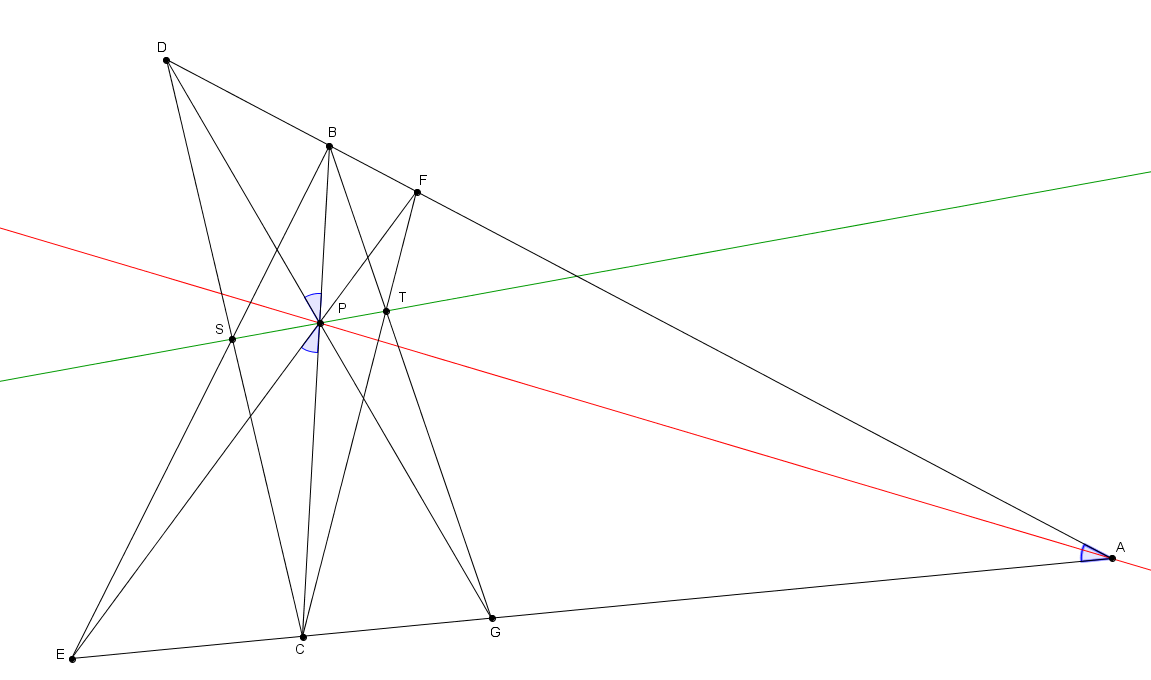
\includegraphics[width=0.80\textwidth]{Senkrecht1}
\end{figure}
Wir bemerken nun, dass sich $AP,BE$ und $CD$ genau dann in einem Punkt schneiden, wenn die Geraden $AP$ und $PT$ zusammenfallen. Und dies ist genau dann der Fall, wenn $T$ auf der Strecke $AP$ liegt.\\
Es genügt also zu zeigen, dass $AP$ und $BC$ genau dann senkrecht aufeinander stehen, wenn $T$ auf der Strecke $AP$ liegt.\\
Wir stellen noch fest, dass wegen $\angle FPB=\angle EPC=\angle BAC$ das Viereck $PCAF$ ein Sehnenviereck ist und aus analogen Gründen auch $PGAB$.\\
\begin{enumerate}
\item Wenn $AP$ und $BC$ senkrecht aufeinander stehen, dann liegt $T$ auf der Strecke $AP$: Nach dem Peripheriewinkelsatz an oben gefundenen Sehnenvierecken gilt $\angle AGB=\angle APB=90^\circ$ und $\angle CFA=\angle CPA=90^\circ$, also sind $BG$ und $CF$ Höhen im Dreieck $ABC$. Das bedeutet, dass $T$ der Höhenschnittpunkt ist und somit auch auf der Höhe durch $A$ liegt. Dies ist aber gerade die Strecke $AP$, und somit liegt $T$ auf $AP$.\\
\begin{figure}[h]
\centering 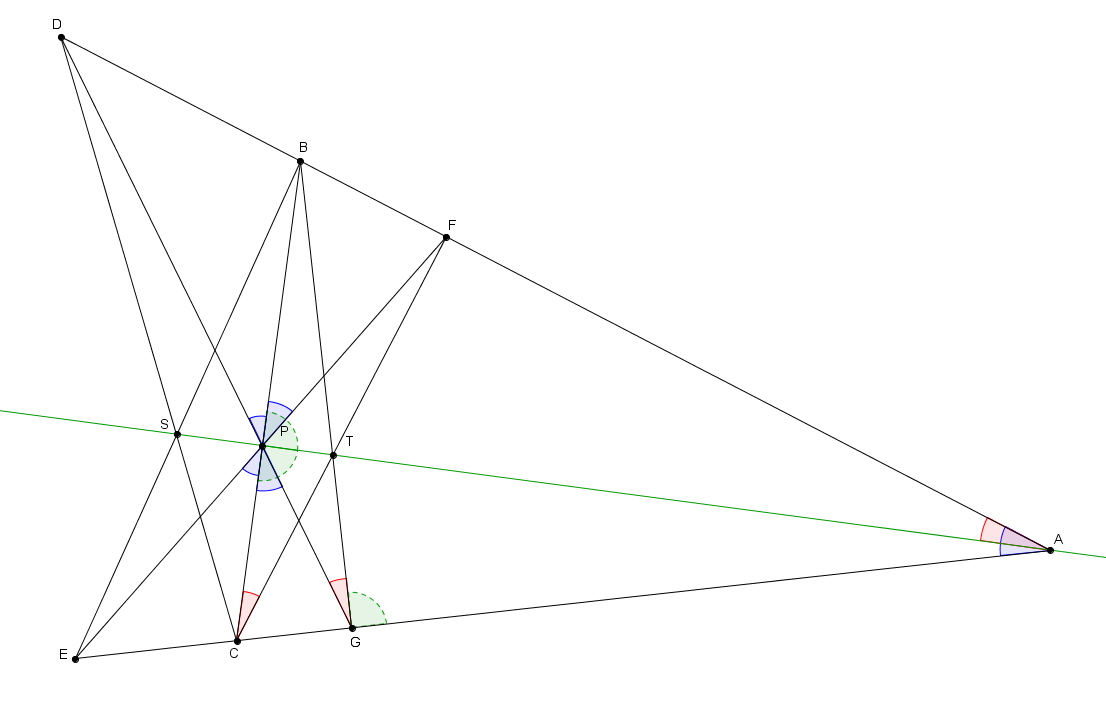
\includegraphics[width=0.80\textwidth]{Senkrecht2}
\end{figure}
\item Wenn $T$ auf der Strecke $AP$ liegt, dann stehen $AP$ und $BC$ senkrecht aufeinander: Nach dem Peripheriewinkelsatz gilt $\angle TCP=\angle FCP=\angle FAP=\angle BAP=\angle BGP=\angle TGP$, woraus folgt, dass auch $CGTP$ ein Sehnenviereck ist. Hiermit erhalten wir nun:
\[
\angle CPT=\angle AGT=\angle AGB=\angle APB=\angle TPB
\]
Daraus folgt sofort, dass $AP$ und $BC$ senkrecht aufeinander stehen und wir sind fertig.
\end{enumerate}

    \item[\textbf{6.}] Montrer qu'il n'existe pas deux nombres entiers naturels distincts tels que leur moyenne harmonique, géométrique, arithmétique et quadratique soient toutes des nombres entiers naturels.\\
	
\textit{Solution:}\\
Supposons que $a,b$ satisfont les hypothèses. Posons $d=pgcd(a,b)$ et $a=dx$, $b=dy$.
Ainsi, on voit par la moyenne arithmétique que $x,y$ sont impairs, et par la moyenne géométrique, comme $(x,y)=1$, que $x,y$ sont des carrés parfaits. Pour $x=x_1^2$ et $y=y_1^2$, la moyenne quadratique nous dit qu'il doit exister un entier naturel $z$ tel que $x_1^4+y_1^4=2z^2$. \\
Or, cette équation est équivalente (comme $x_1,x_2$ sont impairs) à $(\frac{x_1^4-y_1^4}{2})^2=z^4-(x_1y_1)^4$. Donc il faut trouver des nombres naturels $p,q,r$ tels que 
\[
r^2=p^4-q^4
\]
Traitons cette équation en toute généralité. On peut supposer SDPG que $(p,q)=1$, on sait qu'il doit exister une solution minimale $(p_0,q_0,r_0)$ (telle que $p_0q_0r_0$ est minimal par exemple). 2 cas se présentent à nous :

\begin{itemize}
    \item[1)] Si $q$ est pair, par les triplets de Pythagore, il existe deux entiers $m,n$ premiers entre eux tels que $p^2=m^2+n^2$ et $q^2=2mn$. De nouveau par les triplets de Pythagore, il existe $m_1, n_1$ tel que $mn=2m_1n_1(m_1^2-n_1^2)$. Ainsi, $(\frac{q}{2})^2=m_1n_1(m_1^2-n_1^2)$. Comme $m_1$ et $n_1$ sont premiers entre eux, les trois facteurs de l'expression précédente sont des carrés parfaits, disons $m_1=p_1^2, m_2=q_1^2$ et $m_1^2-n_1^2=r_1^2$. Ainsi,\[r_1^2=p_1^4-q_1^4\]
On a donc réussi à créer une solution plus petite que la solution minimale vu que $p_1q_1r_1=\frac{q}{2}<pqr$, contradiction.
    \item[2)] Si $q$ est impair, on fait de męme : $p^2=m^2+n^2$ et $q^2=m^2-n^2$. Donc $(pq)^2=m^4-n^4$. Or, $pqr=2mnpq>mnpq$. Donc nous avons dans ce cas aussi construit une solution plus petite, contradiction.
\end{itemize}

    \item[\textbf{7.}]
Die zwei Kreise $\omega_1$ und $\omega_2$ berühren sich im Punkt $A$ und liegen innerhalb des Kreises $\Omega$. Dabei berührt $\omega_1$ den Kreis $\Omega$ im Punkt $B$ und $\omega_2$ berührt $\Omega$ im Punkt $C$. Die Gerade $AC$ schneidet $\omega_1$ ein weiteres Mal im Punkt $D$.\\
Zeige, dass $DBC$ ein rechtwinkliges Dreieck ist, falls $A$, $B$ und $C$ nicht auf einer Geraden liegen.\\

\textit{1. Lösung:}\\
Sei $O$ der Mittelpunkt von $\Omega$ und seien $M_1$ und $M_2$ die Mittelpunkte von $\omega_1$ respektive $\omega_2$. Nach Voraussetzung liegen $M_1,A,M_2$ auf einer Geraden. Dasselbe gilt auch für $B,M_1,O$ und $C,M_2,O$.\\
Sei $E$ der zweite Schnittpunkt von $BC$ und $\omega_1$. Weiter definieren wir $\alpha=\angle M_2CA$ und $\beta=\angle ACB$. Nun gilt:
\[\angle M_1DA=\angle DAM_1=\angle CAM_2=\angle M_2CA=\alpha\]
\[\angle M_1EB=\angle EBM_1=\angle CBO=\angle OCB=\alpha+\beta\]
Wegen $\angle M_1EB=\angle M_2CB$ sind die Strecken $M_1E$ und $M_2C$ parallel. Dann ist $\angle EM_1A$ als Wechselwinkel aber gerade gleich gross wie $\angle OM_2A$, und der ist nach dem Aussenwinkelsatz am Dreieck $ACM_2$ $2\alpha$.\\
Hieraus folgt nun $\angle EM_1A+\angle AM_1D=2\alpha+(180^\circ-2\alpha)=180^\circ$, das heisst $E,M_1,D$ liegen auf einer Geraden. Dann ist $B$ aber ein Punkt auf dem Thaleskreis über $ED$ und somit gilt $\angle EBD=90^\circ$.\\
\begin{figure}
\centering 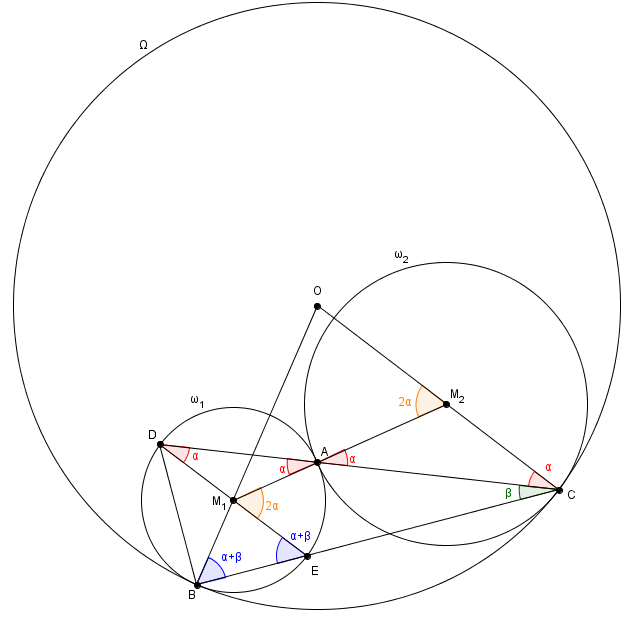
\includegraphics[trim=2cm 0cm 0cm 6cm, clip = true, width=0.90\textwidth]{Aufgabe7_1}
\end{figure}

\textit{2. Lösung:}\\
Sei $E$ der zweite Schnittpunkt von $AB$ und $\omega_2$. Da sich $\omega_1$ und $\omega_2$ in $A$ berühren, existiert eine zentrische Streckung mit Streckzentrum $A$, die den Kreis $\omega_1$ auf $\omega_2$ abbildet. Dabei wird $B$ auf $E$ und $D$ auf $C$ abgebildet, folglich sind die Dreiecke $ADB$ und $ACE$ ähnlich. Ausserdem folgt daraus auch, dass $BD$ und $CE$ parallel sind.\\
Seien $D'$ und $A_1$ die weiteren Schnittpunkte von $\Omega$ mit $BD$ respektive $BA$. Da sich $\omega_1$ und $\Omega$ in $B$ berühren, existiert eine zentrische Streckung mit Streckzentrum $B$, die $D$ auf $D'$ und $A$ auf $A_1$ abbildet. Somit sind die Dreiecke $ADB$ und $A_1D'B$ ähnlich.\\
Analog definieren wir $E'$ und $A_2$ als die weiteren Schnittpunkte von $\Omega$ mit $CE$ respektive $CA$. Hier erhalten wir, dass die Dreiecke $ACE$ und $A_2CE'$ ähnlich sind.\\
Insgesamt können wir schliessen, dass die Dreiecke $A_1D'B$ und $A_2CE'$ ähnlich sind. Da beide Dreiecke denselben Umkreisradius besitzen, sind sie sogar kongruent. Entsprechende Seiten sind somit gleich lang, was uns $BD'=CE'$ liefert. Wie wir bereits festgestellt haben, sind $BD$ und $CE$ parallel, also auch $BD'$ und $CE'$. $BD'$ und $CE'$ sind daher parallele Sehnen in $\Omega$ mit gleicher Länge, woraus wir folgern können, dass $BCE'D'$ ein Rechteck ist. Die Aussage folgt nun sofort.

\begin{figure}
\centering 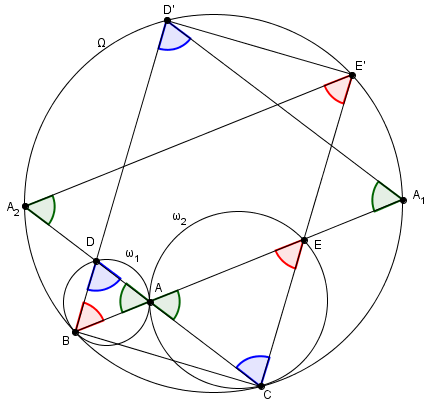
\includegraphics[width=0.60\textwidth]{Aufgabe7_2}
\end{figure}

\item[\textbf{8.}] 
Finde alle Funktionen $f:\R \rightarrow \R$, sodass für alle $x,y \in \R$ gilt:
\[
f(f(x)-y^2)= f(x^2) +y^2f(y) -2f(xy)
\]

\textit{Lösung}\\
Zuerst setzten wir $x=0$ und erhalten
\[
f(f(0)-y^2) = y^2f(y) -f(0).
\]
Nun ändert sich die linke Seite offensichtlich nicht, wenn wir $y$ durch $-y$ ersetzten, also auch nicht die rechte und wir erhalten $y^2f(y) = y^2f(-y)$ für alle $y \in \R$ und somit auch 
\begin{eqnarray}
f(y) = f(-y).
\end{eqnarray}	
Als nächstes setzten wir $x=y=1$ und erhalten $f(f(1)-1) =0$, also hat $f$ eine Nullstelle $a \in \R$. Nun erhalten wir mit $x=y=a$ die Gleichung $f(-a^2)=-f(a^2)$ und somit wegen $(1)$ auch $f(a^2)=0$. Mit $x=a$ und $y=0$ sehen wir $f(0)=f(a^2)-2f(0)$ und somit $f(0)=0$.\\ 
Nun setzten wir $x=0$, verwenden wieder $(1)$ und erhalten
\begin{eqnarray}
f(y^2)=y^2f(y).
\end{eqnarray}
Mit $x=y$ und $(2)$ sehen wir, dass die rechte Seite sich zu $0$ addiert und somit folgt für alle $x \in \R$
\begin{eqnarray}
f(f(x)-x^2)=0.
\end{eqnarray}
Die Idee ist nun, dass $f$ den Wert $0$ entweder nur bei $0$ annimmt oder sont konstant $0$ sein muss. Dazu nehme an es gibt eine reelle Zahl $b\neq 0$ mit $f(b)=0$, dann gilt wegen $(2)$ auch $f(b^2)=0$ und wenn wir schliesslich $x=b$ in die ursprüngliche Gleichung einsetzen und $(1)$ und $(2)$ verwenden finden wir für alle $y\in\R$
\[
f(by)=0.
\]
Nach Annahme ist $b\neq 0$ und somit kann $by$ jeden reellen Wert annehmen und wir sehen, dass $f(x)=0$ für alle $x\in\R$ gelten muss, was in der Tat eine Lösung ist.\\
Falls nun kein $b\neq 0$ mit $f(b)=0$ existiert folgt aus $(3)$ sofort, dass $f(x) = x^2$ für alle $x \in \R$ gelten muss. Man sieht leicht, dass dies in der Tat eine Lösung ist. 

    \item[\textbf{9.}]
Sei $n$ eine natürliche Zahl und $A=\{P_1,P_2,\dots,P_n\}$ eine Menge von $n$ Punkten in der Ebene, von denen keine drei auf einer Geraden liegen. Ein \textit{Weg durch $A$} besteht aus $n-1$ Strecken $P_{\sigma(i)}P_{\sigma(i+1)}$ für $i=1,\dots,n-1$, wobei $\sigma$ eine Permutation von $\{1,2,\dots,n\}$ ist, sodass sich keine zwei Strecken überkreuzen.\\
Zeige, dass die Anzahl verschiedener Wege durch $A$ genau dann minimal ist, wenn die Punkte aus $A$ ein konvexes $n$-Eck bilden.\\

\textit{Lösung}\\
Betrachte die konvexe Hülle der Punkte in $A$ und wähle einen Punkt $P_{\sigma(1)}$ davon aus. Nun betrachte die konvexe Hülle der restlichen $n-1$ Punkte und verbinde $P_{\sigma(1)}$ mit einem Punkt $P_{\sigma(2)}$ auf der neuen konvexen Hülle, \emph{ohne diese zu schneiden}. Wir wiederholen nun dieses Verfahren:

		Betrachte den Teilweg $W=P_{\sigma(1)} P_{\sigma(2)} \ldots P_{\sigma(i)}$ durch $A$ der Länge $i$, und bezeichne mit $C_i$ und $C_{i+1}$ die konvexen Hüllen der Mengen $A \setminus \left\{ P_{\sigma(1)}, \ldots, P_{\sigma(i-1)} \right\}$, respektive $A \setminus \left\{ P_{\sigma(1)}, \ldots, P_{\sigma(i)} \right\}$. Seien $P$ und $Q$ die Nachbarn von $P_{\sigma(i)}$ auf $C_i$. Dann kann man $P_{\sigma(i)}$ genau mit denjenigen Punkten in $C_{i+1}$ verbinden, welche im Dreieck $\triangle P_{\sigma(i)}PQ$ liegen. Nun machen wir die folgenden drei Beobachtungen:
		\begin{itemize}
			\item	Es gibt mindestens zwei solcher Punkte (nämlich $P$ und $Q$).
			\item	Falls alle Punkte aus $A$ zu Beginn weg ein konvexes $n-$Eck bilden, so sind $P$ und $Q$ die einzigen dieser Punkte.\\
				(Da $C_i$ in diesem Fall alle Punkte aus $A \setminus \left\{ P_{\sigma(1)}, \ldots, P_{\sigma(i-1)} \right\}$ enthält.) 
			\item	Verbindet man $P_{\sigma(i)}$ mit einem anderen Punkt in $C_{i+1}$ (das heisst einem Punkt \emph{ausserhalb} von $\triangle P_{\sigma(i)}PQ$), so liegen $P$ und $Q$ auf unterschiedlichen Seiten der Diagonale $P_{\sigma(i)}P_{\sigma(i+1)}$ und können demzufolge nicht mehr beide erreicht werden.
		\end{itemize}

		Falls alle Punkte zu Beginn ein konvexes $n-$Eck bilden, haben wir demzufolge $n$ Möglichkeiten, $P_{\sigma(1)}$ zu wählen. Danach gibt es in jeweils genau zwei Möglichkeiten, den nächsten Punkt zu wählen, insgesamt also $2^{n-2}$ Möglichkeiten. Da wir Wege nicht doppelt zählen wollen (in jede Richtung einmal), erhalten wir insgesamt $n\cdot 2^{n-3}$ verschiedene Wege durch $A$.

		Nun gibt es zwei Möglichkeiten, um zu zeigen, dass die Anzahl verschiedener Wege durch $A$ strikt grösser ist als $n2^{n-3}$, falls die Punkte aus $A$ kein konvexes $n-$Eck bilden.

		\begin{figure}[ht!]
			\centering
			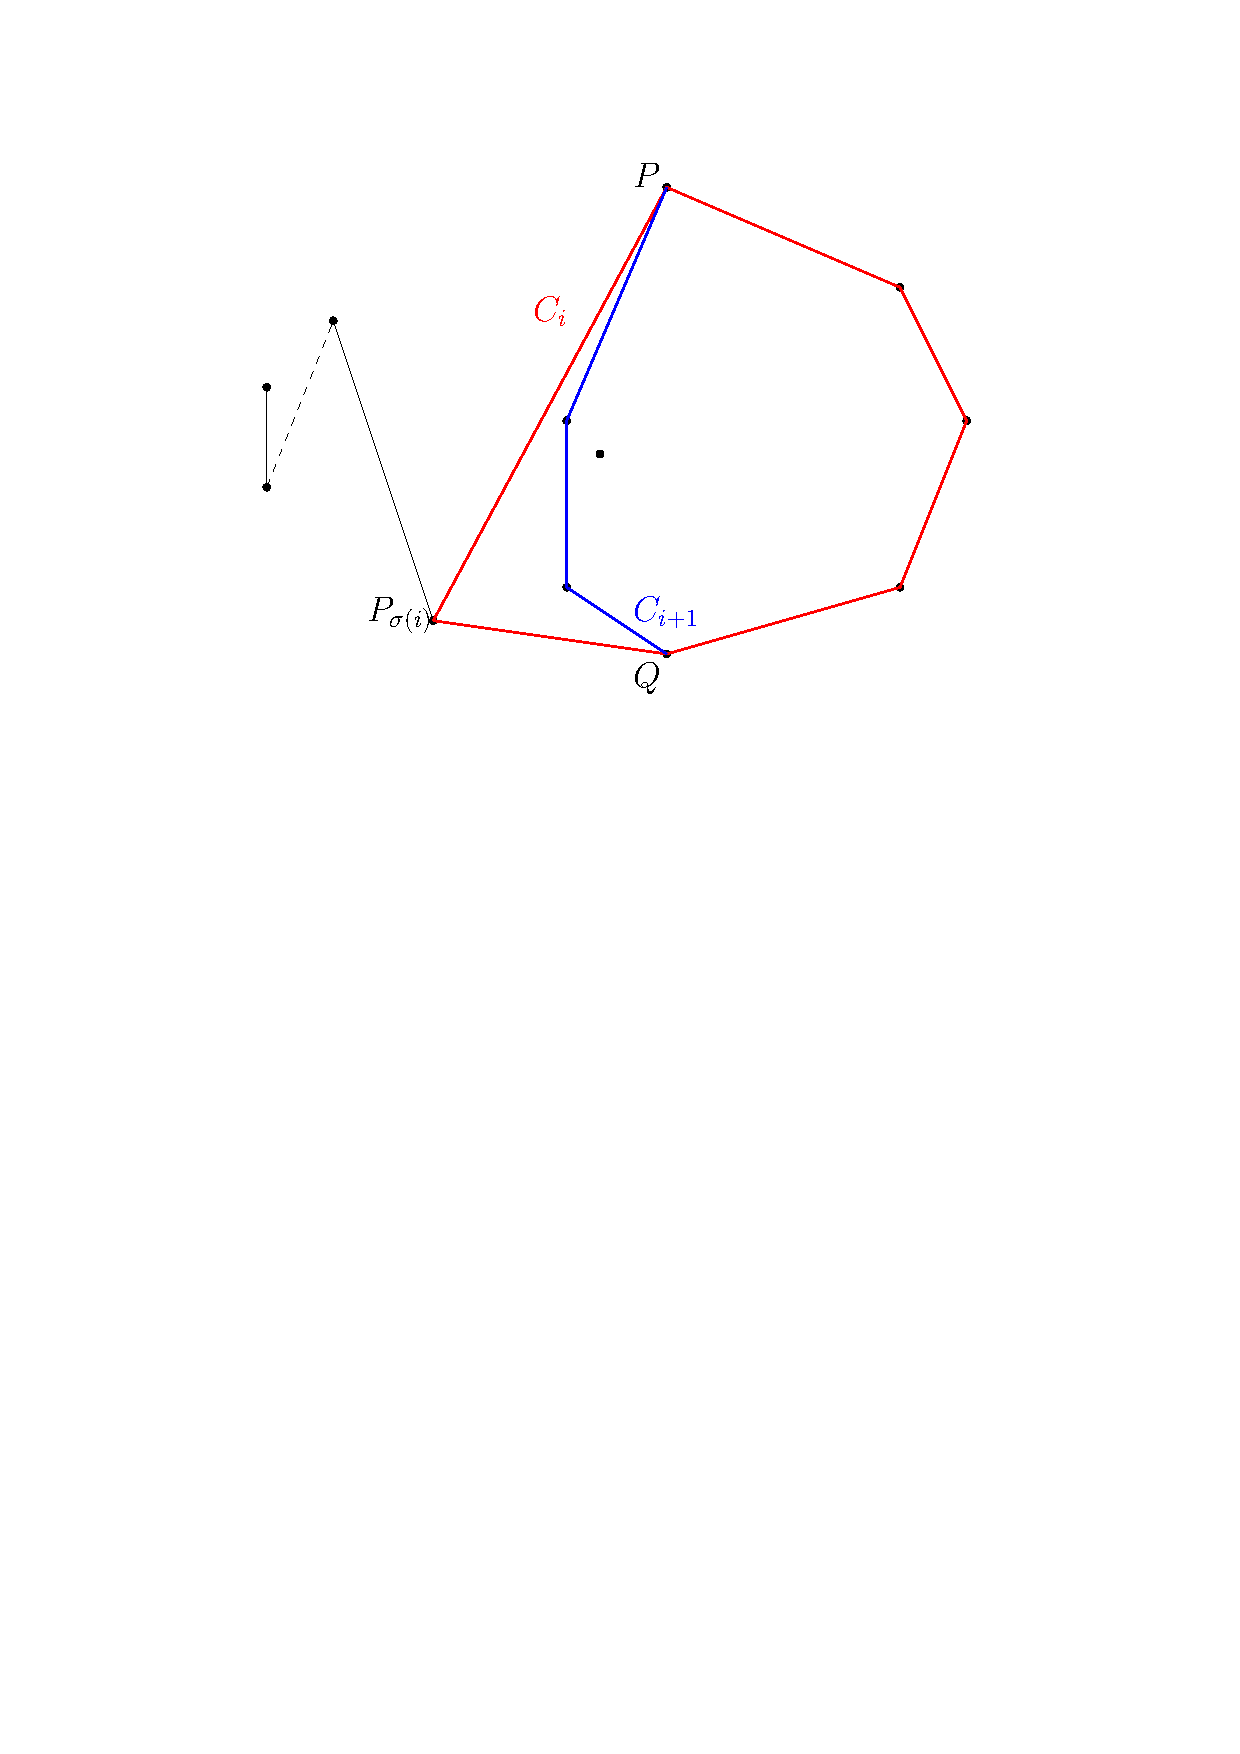
\includegraphics[width=0.5\linewidth]{fig-loesung9.pdf}
			\caption{$P_{\sigma(i)}$ kann mit 4 Punkten verbunden werden ($a_{i+1}=2$).}
		\end{figure}		
		
		
		\textit{Lösung 1}\\
		Sei $k<n$ die Anzahl Punkte aus $A$ auf der konvexen Hülle $C_1$ von $A$. Mit $a_{i+1}$ bezeichnen wir die Anzahl Punkte von $C_{i+1}$ im \emph{Innern} des Dreiecks $\triangle P_{\sigma(i)}PQ$. Dann gibt es mindestens $k\cdot \frac{(2+a_2)(2+a_3)\cdots(2+a_{n-1})}{2}$ Wege durch $A$. Jeder neu verbundene Punkt $P_{\sigma(i+1)}$ muss zum Zeitpunkt, zu welchem er verbunden wird, auf der konvexen Hülle liegen. Das heisst, der Punkt $P_{\sigma(i+1)}$ liegt entweder bereits zu Beginn auf $C_1$, oder er kommt erst später dazu, wird also durch mindestens ein $a_{j,\ j\leq i+1}$ gezählt.  Da ein Weg alle Punkte aus $A$ verbindet (also auch die $n-k$ Punkte im Innern von $C_1$), erhalten wir $\sum_{i=2}^{n-1}a_i \geq n-k$. Hiermit und wegen $k>2$ gilt:
		\[	k\cdot \frac{(2+a_2)(2+a_3)\cdots(2+a_{n-1})}{2} \geq k2^{n-3}+k(n-k)2^{n-4}>n2^{n-3}.	\]

		\textit{Lösung 2}\\
		Sei $M$ ein Punkt auf der konvexen Hülle. Zuerst zählen wir wie vorher die Anzahl Wege, die $M$ als Startpunkt haben. Da die Punkte in $A$ nicht in konvexer Lage sind, gibt es einen Zeitpunkt $i$, zu welchem das Dreieck $\triangle P_{\sigma(i)}PQ$ mindestens drei Punkte aus $C_{i+1}$ enthält. Es gibt also strikt mehr als $2^{n-2} = 2\cdot 2^{n-3}$ solcher Wege.

		Nun schätzen wir die Anzahl Wege ab, welche $M$ im Innern haben. Dazu teilen wir mit einer Geraden durch $M$ die restlichen Punkte in $j$ Punkte ($1\leq j\leq n-2$) auf der linken Seite der Geraden und $n-j-1$ Punkte auf der rechten Seite der Geraden auf. Dabei gibt es $n-2$ Möglichkeiten, die Gerade zu wählen. Nun ist $M$ wiederum Startpunkt von zwei Teilwegen: einem Weg auf $j+1$ Punkten auf der linken Seite und einem Weg auf $n-j$ Punkten auf der rechten Seite der Geraden. Zusammen erhalten wir nun wie vorhin $\geq (n-2) \cdot 2^{(j+1)-2} \cdot 2^{(n-j)-2} = (n-2)\cdot 2^{n-3}$ Wege.

		Total haben wir also sicher mehr wie $2\cdot 2^{n-3} + (n-2)\cdot 2^{n-3} = n2^{n-3}$ verschiedene Wege durch $A$.
		(\emph{Anmerkung:} Es könnte auch Wege geben, welche jede mögliche Gerade durch $M$ mehrfach kreuzen, diese Wege brauchen wir für die Abschätzung aber nicht.)


    \item[\textbf{10.}]
Ein $7\times 7$ Quadrat ist in $49$ kleine $1\times 1$  Quadrate unterteilt. Zwei Ameisen laufen den Seiten der kleinen Quadrate entlang, wobei jede Ameise ihren eigenen geschlossenen Weg läuft und alle $64$ Eckpunkte der kleinen Quadrate genau einmal besucht. \\
Welches ist die minimale Anzahl Seiten der kleinen Quadrate, über die beide Ameisen laufen?\\

\textit{Lösung}\\
Wir werden zeigen, dass es minimal 16 Seiten gibt, über die beide Ameisen laufen. Dafür zeigen wir zuerst die untere Schranke und dann geben wir eine Konstruktion an.
\begin{enumerate}
\item 1. Schranke: Jede Ameise muss genau 64 Kanten entlang laufen, um alle Punkte einmal zu besuchen und dann noch zum Anfangspunkt zurückzukehren. Die beiden Ameisen zusammen laufen also $64 \cdot 2 = 128$ Kanten entlang. Insgesamt gibt es $8 \cdot 7 \cdot 2 = 112$ verschiedene Kanten. Somit muss es mindestens 16 Kanten geben, entlang derer beide Ameisen gelaufen waren.
\item 2. Konstruktion: Die Ideen waren dabei, dass jede Kante von einer Ameise entlang gelaufe werden muss. Weiter sieht man, dass jede Ameise in den Ecken vorbei muss. Mit einer Mischung von Ordnung und Kreativität findet man nach genug Ausprobieren eine Konstruktion.\\
Abbildung: Eine Ameise läuft der dicken, dunklen Linie entlang. Die andere läuft dem Rand der grauen Fläche entlang.
\end{enumerate}
\mbox{\centering 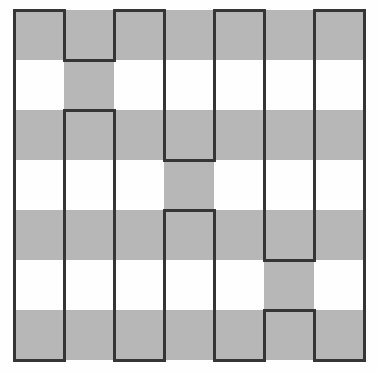
\includegraphics[width=0.60\textwidth]{Ameisen}}

\item[\textbf{11.}] 
Bestimme alle natürlichen Zahlen $n$ mit folgender Eigenschaft: \\
Für alle Primzahlen $p<n$ ist $n-\lfloor \frac{n}{p}\rfloor p$ nicht durch das Quadrat einer natürlichen Zahl grösser als $1$ teilbar.\\
\textit{Bemerkung: Für $x \in \R$ bezeichnet $\lfloor x\rfloor$ die grösste ganze Zahl mit $\lfloor x\rfloor \leq x$.}\\

\textit{Solution}\\
On remarque tout d'abord, que la condition avec la partie entière revient à considérer le reste de la division de $n$ par $p$.\\
Si $n$ n'est pas premier, alors il existe un premier $q<n$ tel que $q|n$ et donc $n-\lfloor \frac{n}{q}\rfloor q = 0$ et en particulier est divisible par un carré.\\
Si $n>13$, alors $n-4$ (qui est impair) ne peut être divisible que par $3$, sinon il existerait un premier $3<q\leq n-4<n$ tel que $n \equiv 4 \pmod q$. Donc $n-4=3^k$.\\
De plus, $n-8$ est aussi impair et ne peut pas être divisible par $3$, car $3|n-4$. Donc, par le même argument, $n-8$ ne peut être divisible que par $5$ et $7$.\\
Quant à $n-9$, il ne peut pas être divible ni par $3$, ni par $5$ (sinon $n \equiv 4 \pmod 5$). Donc il est divisible seulement par $2$ et $7$.\\
Maintenant, $7$ ne peut pas diviser à la fois $n-8$ et $n-9$, donc on a soit $n-8=5^l$, soit $n-9=2^l$. Dans le premier cas on aurait $3^m=4+5^l$ et dans le deuxième $3^m=5+2^l$.\\
En prenant la première équation modulo $8$, on obtient que $m$ doit être pair. Donc $(3^{m/2}+2)(3^{m/2}-2)=5^l$ et on remarque que les deux membres de gauche ne peuvent être des multiples de $5$ en même temps, donc la seule solution est $m=2$ et $l=1$ qui nous mène à $n=13$.\\
Pour le deuxième cas, si $l\geq 3$, alors l'équation n'a pas de solution modulo $8$. Ce qui entraîne la seule solution $m=2$ et $l=2$ qui donne $n=13$.\\
On traite donc les cas $n\leq 13$ à la main et on trouve les uniques solutions $\{ 3,5,7,13 \}$.

\item[\textbf{12.}]
Gegeben sind eine natürliche Zahl $n$ und natürliche Zahlen $a_1,a_2, \dots,a_n$. Wir erweitern die Folge periodisch durch $a_{n+i} = a_i$ für alle $i\geq 1$. Nehme nun an, dass folgende zwei Bedingungen erfüllt sind:
\begin{enumerate}
    \item[(i)] $a_1\leq a_2\leq\dots \leq a_n\leq a_1 +n$.
    \item[(ii)] $a_{a_i} \leq n+i-1$ für $i=1,2\dots,n$.
\end{enumerate}
Zeige, dass gilt:
\[
a_1+a_2+\dots +a_n \leq n^2
\]

\textit{Lösung}\\
Wir wissen, dass $a_1 \le a_{a_1} \le n$ gilt. Für $a_j < i \le a_{j+1}$ haben wir $a_i \le a_{a_{j+1}} \le n+j$ und für $a_{a_1} < i \le n$ haben wir $a_i \le a_n \le a_1+n$.\\
Kombiniert erhalten wir folgende Ungleichungen:

\begin{align*}
a_1+a_2+\dots + a_n= & a_1+a_2+\dots + a_{a_1} + \dots + a_{a_2} + \dots + a_{a_{a_1}} + \dots + a_n  \\
\le & a_1+a_2+\dots +a_{a_1} + \\
& a_{a_2}(a_2-a_1)+\dots + a_{a_{a_1}}(a_{a_1}- a_{a_1-1}) + (n+a_1)(n- a_{a_1}) \\
\le &  a_1+a_2+\dots+  a_{a_1} +\\
& (n+1)(a_2-a_1)+\dots + (n+a_1-1)( a_{a_1}- a_{a_1-1}) + (n+a_1)(n- a_{a_1}) \\
= &n^2
\end{align*}

\end{enumerate}

\end{document}
